\documentclass{beamer}
\usepackage[english]{babel}
\usepackage[utf8]{inputenc}
\usepackage{lmodern}
\usepackage{apacite}

\title{Open Source}
\subtitle{Freedom for a digital world}
\author{William Jagels, Jonathan Terner, and Nikolas Vanderhoof}
\institute{Binghamton University}
\date{April 25, 2016}

\usetheme{Warsaw}
\setbeamertemplate{itemize items}[default]
\setbeamertemplate{enumerate items}[default]
\setbeamertemplate{frametitle}[default][colsep=-4bp,rounded=false,shadow=false]
\setbeamertemplate{section page}
{
  \begin{centering}
    \begin{beamercolorbox}[sep=12pt,center]{part title}
      \usebeamerfont{section title}\insertsection\par
    \end{beamercolorbox}
  \end{centering}
}
\setbeamertemplate{caption}{\raggedright\insertcaption\par}

\begin{document}
\frame{\titlepage}

\section{Overview}\frame{\sectionpage}

\begin{frame}{Overview}
  \begin{column}{.5\linewidth}
    Open Source...
    \begin{itemize}
      \item Benefits users
        \begin{itemize}
          \item Protects liberties
          \item No DRM
        \end{itemize}
      \item Is practical
        \begin{itemize}
          \item No vendor lock in
          \item Extensible
          \item Repurposable
        \end{itemize}
    \end{itemize}
  \end{column}
  \begin{column}{.5\linewidth}
    \begin{itemize}
      \item Is good for the economy
        \begin{itemize}
          \item Free of cost
          \item Open innovation
          \item Skilled community
        \end{itemize}
      \item Is secure
        \begin{itemize}
          \item Community of bug fixers
          \item Provably secure instead of obscurity
        \end{itemize}
    \end{itemize}
  \end{column}
\end{frame}

\section{Summary}\frame{\sectionpage}

\subsection{Principles}
\begin{frame}{The Four Freedoms of Free Software}
  \begin{itemize}
    \item Freedom 0 is the freedom to run the program as you wish
    \item Freedom 1 is the freedom to study the source code and change it,
      so the program does your computing the way you wish
    \item Freedom 2 is the freedom to help others. That's the freedom to
      make exact copies and redistribute them when you wish
    \item Freedom 3 is the freedom to contribute to your community. That's
      the freedom to make copies of your modified versions, if you have made any,
      and then distribute them to others when you wish
  \end{itemize}
\end{frame}


\begin{frame}{The GNU Project and the Free Software Movement}
  \begin{column}{.45\textwidth}
    \begin{itemize}
      \item Stallman launched the Free Software movement in 1983
      \item He developed GNU - GNU's Not Unix
      \item Hacker spirt to joke around about serious issues
      \item Developed for freedom of users
      \item GNU+Linux or GNU/Linux
    \end{itemize}
  \end{column}
  \begin{column}{0.5\textwidth}\raggedleft{}
    \begin{figure}
      
\includegraphics[width=\textwidth]{images/gnu-linux.jpg}
      \caption{\Protect\cite{gnuLinux}}
    \end{figure}
  \end{column}
\end{frame}


\begin{frame}{Free Software and Education}
  \begin{itemize}
    \item Schools must teach exclusively free software
    \item Teaching windows teaches dependence
    \item To become a good programmer, one must read lots of code
    \item Free software fosters sharing and helping
  \end{itemize}
\end{frame}


\subsection{Threats to Freedom}
\begin{frame}{Surveillance}
  \begin{column}{0.45\textwidth}
    \begin{itemize}
      \item Can record anything on a computer
      \item Amazon users identify selves when buying books
      \item Mobile phones transmit location
      \item Need control over software
      \item Computer surveillance centralizes information
    \end{itemize}
  \end{column}
  \begin{column}{0.5\textwidth}\raggedleft{}
    \begin{figure}
      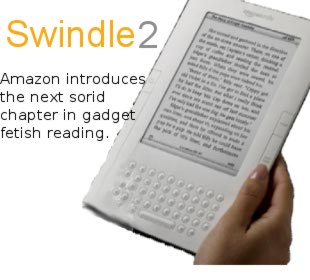
\includegraphics[width=\textwidth]{images/swindle.jpg}
      \caption{\Protect\cite{swindle}}
    \end{figure}
  \end{column}
\end{frame}

\begin{frame}{Censorship}
  \begin{column}{0.45\textwidth}
    \begin{itemize}
      \item Arbitray shutdown of sites in Spain
      \item Denmark secretly blocked sites
      \item A country that imposes censorship is not
        \begin{itemize}
          \item free
          \item legitamte
        \end{itemize}
    \end{itemize}
  \end{column}
  \begin{column}{0.5\textwidth}\raggedleft{}
    \begin{figure}
      
\includegraphics[width=\textwidth]{images/censorship.jpg}
      \caption{\Protect\cite{censorship}}
    \end{figure}
  \end{column}
\end{frame}

\begin{frame}{Restricted Data Formats}
  \begin{itemize}
    \item Prevents interoperability
    \item DRM is digital handcuffs
    \item Only happens in non-free software
    \item VC1, Flash, MP3
  \end{itemize}
\end{frame}

\begin{frame}{Software That Isn't Free}
  \begin{itemize}
    \item Free as in {\it libre\/}
    \item Free software respects a user's freedom
    \item The user controls free software
    \item Backdoor
  \end{itemize}
\end{frame}

\begin{frame}{Internet Services}
  \begin{itemize}
    \item Server could abuse data or take control
    \item Never trust data to a US company - Patriot Act
    \item Do things remotely with your own server
    \item Doing things digitally should not require loss of rights
  \end{itemize}
\end{frame}

\begin{frame}{Computers for Voting}
  \begin{itemize}
    \item Can't trust computers for voting
    \item Neither free or non-free software can be used
    \item If non-free software is used, company controls voting
    \item If free software is used, whoever runs the machine is in control
    \item Ballots can't be recounted with digital voting
  \end{itemize}
\end{frame}

\begin{frame}{The War on Sharing}
  \begin{itemize}
    \item Technology makes it easy to copy published works
    \item Those who have power over distribution do not want sharing
    \item Suing teenages for hundreds of thousands of dollars for sharing
    \item DMCA makes free software that circumvents DRM illegal
    \item Streaming media requires proprietary software
    \item Users should have their own copy of media
  \end{itemize}
\end{frame}

\begin{frame}{Rights in Cyberspace}
  \begin{itemize}
    \item No firm right to do things in cyberspace
    \item Need support of ISP to have website
    \item Need support of payment company to get paid
    \item US government had Amazon cut off service to WikiLeaks
    \item Also had PayPal cut service from WikiLeaks
    \item Need to have same rights in physical and virtual worlds
  \end{itemize}
\end{frame}

\section{Analysis}\frame{\sectionpage}

%first slide
\subsection{Basis}
\begin{frame}{Stallman's Argument: Basis}
  \begin{column}{0.5\textwidth}
    \begin{itemize}
      \item A deontological standpoint
      \item Stallman as an ethical essentialist
        \begin{itemize}
          \item proprietary software
          \item restricted data formats
          \item internet services
          \item surveillance
        \end{itemize}
        \begin{itemize}
          \item ``always bring up [free software] as an ethical issue''~\cite[para. 63]{rms2011}
        \end{itemize}
    \end{itemize}
  \end{column} %\hfill
  \begin{column}{0.45\textwidth}\raggedleft
    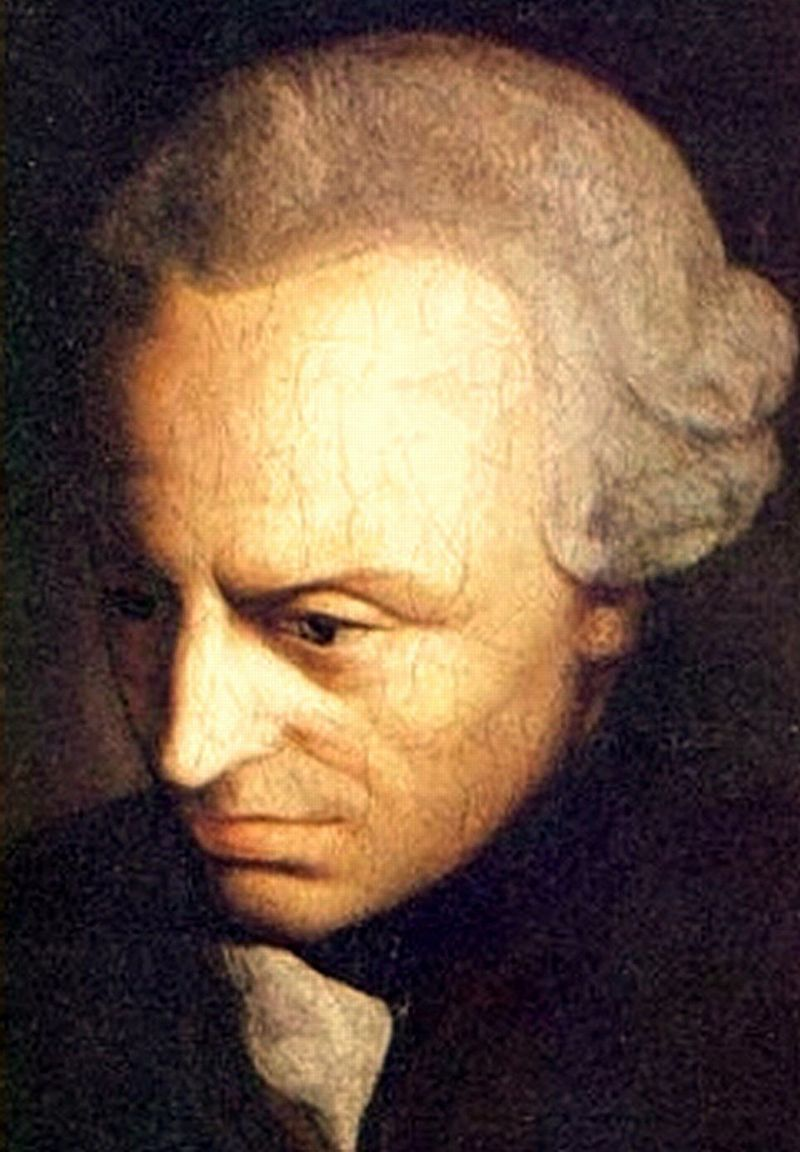
\includegraphics[width = 0.75\textwidth]{kant.jpg}
  \end{column}
\end{frame}


\subsection{Logos}
\begin{frame}{Stallman’s Argument: Logos}
  \begin{itemize}
    \item Deductive reasoning
      \begin{itemize}
        \item tobacco and proprietary software comparison~\cite[para. 55]{rms2011}
      \end{itemize}
    \item Contradictory premises
      \begin{itemize}
        \item dismissing economics of free digital society (para. 34)
        \item later addressing economics of digital media (para. 109)
      \end{itemize}
  \end{itemize}
\end{frame}

\subsection{Pathos}
\begin{frame}{Stallman’s Argument: Pathos}
  \begin{itemize}
    \item Use of strong characterizations
      \begin{itemize}
        \item ``Computers are Stalin’s dream''~\cite[para. 3]{rms2011}
        \item All DRM should be illegal (para. 30)
      \end{itemize}
    \item Strong appeals to tradition
      \begin{itemize}
        \item values derived from a non-digital society
        \item Amazon Kindle (para. 98)
      \end{itemize}
    \item Calls Amazon Kindle (para. 98)
      \begin{itemize}
        \item an immediate end to digital surveillance
        \item “you can’t wait until there is another dictator” (para. 13)
      \end{itemize}
  \end{itemize}
\end{frame}


\section{Practical Advantages of Open Source}\frame{\sectionpage}

\begin{frame}{Software for Freedom vs. Freedom for Software}
    \begin{itemize}
      \item Needs fulfilled by free software
        \begin{itemize}
          \item a need for software
          \item a need for ethical software and practices
        \end{itemize}
      \item Stallman's emphasis on a ``free digital society''
      \item Consequentialist stance on free software
        \begin{itemize}
          \item open source vs.\ free software
          \item a less radical approach
          \item weighing the utility of open source
          \item need-driven software~\cite[p. 17]{bisson}
        \end{itemize}
    \end{itemize}
\end{frame}

%%% include a citation for mill.jpg from https://en.wikipedia.org/wiki/John_Stuart_Mill


\begin{frame}{GNU + Linux, GNU/Linux}
  \begin{column}{0.5\textwidth}
    \begin{itemize}
      \item The GNU operating system
        \begin{itemize}
          \item ``written for your freedom''~\cite[para. 48]{rms2011}
        \end{itemize}
      \item The need for a kernel
        \begin{itemize}
          \item 1990: GNU Hurd
          \item 1991: Linux
        \end{itemize}
      \item Fusion of Linux and GNU
        \begin{itemize}
          \item GNU + Linux, or just Linux?
          \item Torvalds vs. Stallman
        \end{itemize}
    \end{itemize}
  \end{column}
  \begin{column}{0.5\textwidth}\raggedleft{}
    \begin{figure}
      
\includegraphics[width = 0.50\textwidth]{images/tux.png}
      
\includegraphics[width = 0.50\textwidth]{images/gnu.png}
      \caption{\Protect\cite{tux}, \Protect\cite{gnu}}
    \end{figure}
  \end{column}
\end{frame}

%%% include a citation for tux.png from https://en.wikipedia.org/wiki/Tux
%%% include a citation for gnu,png from https://en.wikipedia.org/wiki/GNU



\begin{frame}{Linux: Open Source Success Principles}
  \begin{itemize}
    \item Using / creating the best tools for the job
    \item Not started with open source in mind~\cite[3:30]{torvalds}
    \item Open source contributions
      \begin{itemize}
        \item GPL and copyleft
        \item Collaborative efforts and development
        \item Formation of a communities around open-source code
      \end{itemize}
    \item Flexibility
      \begin{itemize}
        \item Availability of source code promotes reuse
        \item power saving on Linux cellphone benefit Linux supercomputers~\cite[11:34]{zemlin}
      \end{itemize}
  \end{itemize}
\end{frame}



\begin{frame}{Another Success Story: Apache HTTP Server}
  \begin{column}{.5\textwidth}
    \begin{itemize}
      \item Most popular web server since 1995
      \item Open source project
      \item Inherited the NCSA Common Gateway Interface.
      \item Repurposed software components
        \begin{itemize}
          \item enabling efficient software development~\cite[p. 17]{bisson}
        \end{itemize}
    \end{itemize}
  \end{column}
  \begin{column}{0.5\textwidth}\raggedleft{}
    \begin{figure}
      \def\svgwidth{0.5\columnwidth}
      \input{images/feather.pdf_tex}
      \caption{\Protect\cite{apache}}
    \end{figure}
  \end{column}
\end{frame}

%% include a citation for apache.png from https://en.wikipedia.org/wiki/Apache_HTTP_Server



\begin{frame}{Preventing Obsolescence}
  \begin{itemize}

    \item Vendor lock-in
      \begin{itemize}
        \item warned against by Stallman~\citeyear[para. 54]{rms2011}
      \end{itemize}
    \item Proprietary software creates vendor dependency
      \begin{itemize}
        \item maintenance
        \item updates
        \item support
      \end{itemize}
    \item Case Study: Electronic voting machines~\cite[p. 916]{colannino}
      \begin{itemize}
        \item migration to electronic voting machines
        \item software escrow
        \item code was licensed for testing, not deployment.
      \end{itemize}
  \end{itemize}
\end{frame}


\begin{frame}{Quality Assurance}
  \begin{column}{.6\textwidth}
    \begin{itemize}
      \item Linus's Law
        \begin{itemize}
          \item 6,782 lines of code added/subtracted from Linux daily~\cite[12:03]{zemlin}
        \end{itemize}
      \item Software peer-review
      \item Core developers and user developers
      \item Mozilla bug reports~\cite[p. 352]{wang}
        \begin{itemize}
          \item value differences
          \item skill differences
          \item reciprocal skill transfer
          \item disorganization preventable
        \end{itemize}
    \end{itemize}
  \end{column}
  \begin{column}{.4\textwidth}\raggedleft{}
    \begin{figure}
      \def\svgwidth{0.75\columnwidth}
      \input{images/firefox.pdf_tex}
      \caption{\Protect\cite{firefox}}
    \end{figure}
  \end{column}
\end{frame}

%%% include a citation for fox.png taken from https://en.wikipedia.org/wiki/Firefox

\section{Economic Advantages of Open Source}\frame{\sectionpage}

\subsection{Open Source in Action}
\begin{frame}{Apache Web Server}
  \begin{itemize}
    \item 66\% of major sites~\cite[p~696]{powell}
    \item Web server development is expensive
    \item Lowers requirements for web companies
    \item Allows publication of ideas and research
  \end{itemize}
\end{frame}

\begin{frame}{Open Simulator}
  \begin{column}{0.45\textwidth}
    \begin{itemize}
      \item Open entrepreneurship case study
      \item Powerful developer network
      \item Used to start software companies
      \item Sharing benefits all parties
      \item\cite{yetis}
    \end{itemize}
  \end{column}
  \begin{column}{0.5\textwidth}\raggedleft{}
    \begin{figure}
      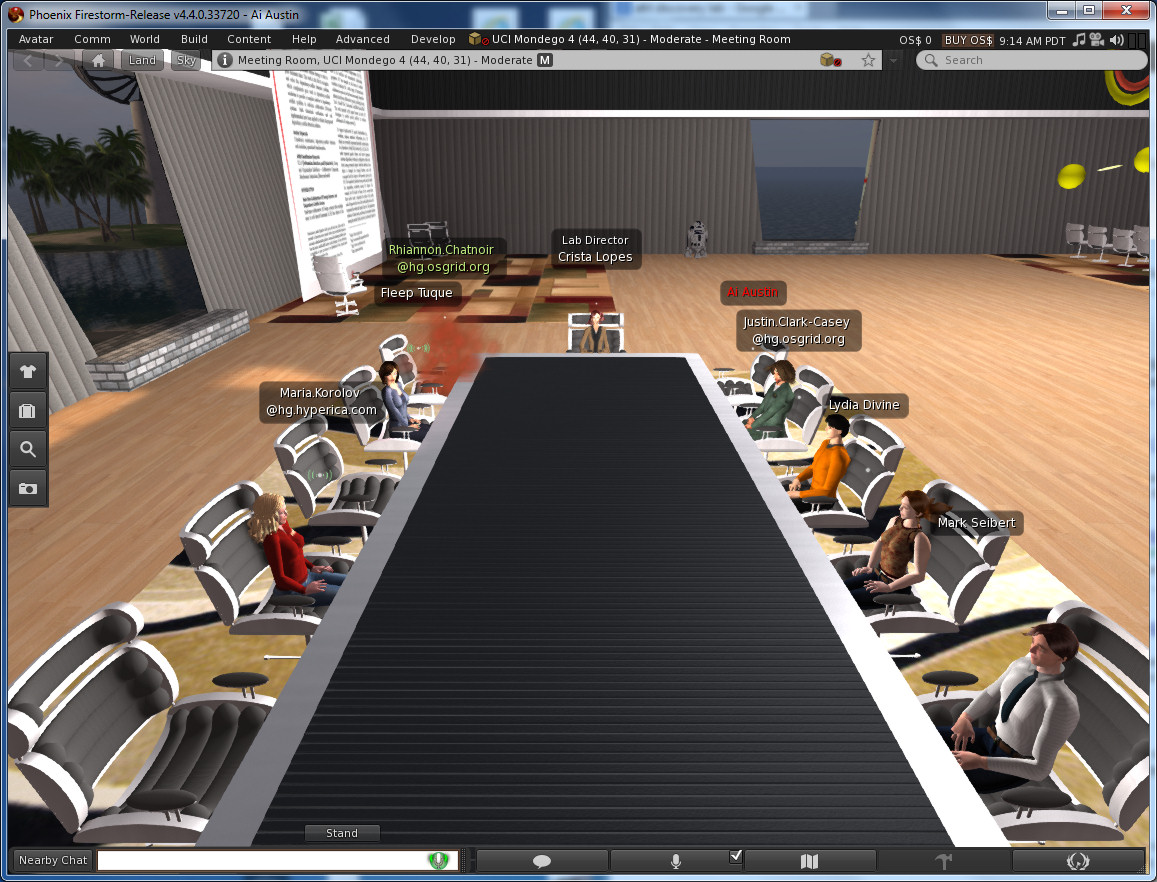
\includegraphics[width=\textwidth]{images/opensim.jpg}
      \caption{\Protect\cite{opensim}}
    \end{figure}
  \end{column}
\end{frame}

\subsection{Open Source in Established Companies}
\begin{frame}{Red Hat}
  \begin{itemize}
    \item \$524M in revenue last quarter~\cite[p.~24]{redhat}
    \item Red Hat Enterprise Linux
      \begin{itemize}
        \item ``Free'' alternative CentOS
      \end{itemize}
    \item Support \& Certifications
    \item Software licensed by GNU GPL
    \item Open technologies (ex. GlusterFS)
  \end{itemize}
\end{frame}

\begin{frame}{id Software}
  \begin{itemize}
    \item Creators of Doom and Quake
    \item Example of delayed open source
    \item Doom engine
      \begin{itemize}
        \item Cutting edge technology when released
        \item Eventually outperformed by competitors
        \item Open sourced engine 1997
        \item Continued to sell content packs for engine
        \item\cite[p.~1188]{caulkins}
      \end{itemize}
    \item Makes economic sense for companies to open source
    \item\cite{caulkins}
  \end{itemize}
\end{frame}

\subsection{Economic Benefits}
\begin{frame}{Economic Benefits}
  \begin{itemize}
    \item Efficient use of human resources
    \item Reuse of works
    \item Shared knowledge
    \item Lower costs
    \item Greater quality of living
    \item Powerful community
  \end{itemize}
\end{frame}

\section{Security Differences between Open Source and Closed Source}\frame{\sectionpage}

\subsection{Security Models}
\begin{frame}{Security Through Obscurity}
  \begin{itemize}
    \item Malicious hackers cannot see source
    \item Any code found is obfuscated
    \item In-house code reviews find bugs
    \item Developers have time to correct bugs
  \end{itemize}
\end{frame}

\begin{frame}{Security Through Transparency}
  \begin{itemize}
    \item Community will find bugs
    \item Developers less likely to inset malicious code
    \item Users that find bugs can propose fixes quickly
  \end{itemize}
\end{frame}

\subsection{Vulnerability Comparison}
\begin{frame}{Microsft Office and Apache OpenOffice}
  \begin{itemize}
    \item Microsoft Office had 108 total vulnerabilities
    \item OpenOffice had only 16
    \item Similar number of low severity vulnerabilites as listed by CVE
    \item Microsoft had 7 times as many medium and high severity ones
    \item Numbers could be influenced by speed of Apache's patches
    \item\cite{kadura}
  \end{itemize}
\end{frame}

\subsection{Types of Vulnerability}
\begin{frame}{Source Dependent Attacks}
  \begin{column}{0.45\textwidth}
    \begin{itemize}
      %Source dependent - can be done without seeing source, but harder
      \item Buffer Overflow
      \item SQL Injection
      \item Patch Reverse Engineering
      \item\cite{clarke}
    \end{itemize}
  \end{column}
  \begin{column}{0.5\textwidth}\raggedleft{}
    \begin{figure}
      
\includegraphics[width=\textwidth]{images/adobe.jpg}
    \end{figure}
  \end{column}
\end{frame}

\begin{frame}{Source Independent Attacks}
  \begin{itemize}
    \item User Participation
    \item Brute Force
    \item Protocol Vulnerability
    \item Inside Jobs
    \item\cite{clarke}
  \end{itemize}
\end{frame}

\section{Conclusion}\frame{\sectionpage}

\subsection{Summary}
\begin{frame}{Practical Advantages}
  \begin{itemize}
    \item Open source has practical advantages
    \item Hard to learn about workings of closed source
    \item Open source empowers users
  \end{itemize}
\end{frame}

\begin{frame}{Economics}
  \begin{itemize}
    \item Entrepreneurs can build off OSS
    \item Lowered entry costs foster innovation
    \item Open source business offer value to others
    \item Easier maintenance of legacy code
  \end{itemize}
\end{frame}


\begin{frame}{Security}
  \begin{itemize}
    \item Gives users confidence
    \item Active community minimizes vulnerabilities
    \item Same community deters malicious code
  \end{itemize}
\end{frame}

\subsection{Closing Thoughts}
\begin{frame}{Closing Thoughts}
  \begin{itemize}
    \item Stallman's ideas are not as radical as they seem
    \item Open source promotes freedom and learning
    \item Gives developers a starting point
    \item Suited for tinkerers
    \item Helps users feel involved and invested
  \end{itemize}
\end{frame}


\begin{frame}[allowframebreaks]{References}
  \bibliographystyle{apacite}
  \bibliography{open-source-piracy}
\end{frame}
\end{document}
